\documentclass[a4paper,12pt,titlepage]{article}
\usepackage[encapsulated]{CJK}
\usepackage{ucs}
\usepackage[utf8x]{inputenc}
\newcommand{\cntext}[1]{\begin{CJK}{UTF8}{gbsn}#1\end{CJK}}
\newcommand{\supercite}[1]{\textsuperscript{\cite{#1}}}
\usepackage[left=2.54cm,right=2.54cm,top=2.54cm,bottom=2.54cm]{geometry}
\usepackage[hidelinks]{hyperref}
\usepackage{color,xcolor,times,graphicx,graphics,fancyhdr,listings,subfigure,lastpage,setspace,algorithm2e,mathtools,amsmath,amsfonts,float,wrapfig}
\title{Vp160 Midterm 2 Review Handout}
\author{Wenhao Peng}
\begin{document}
\newcommand{\unit}[1]{\text{ }\mathrm{#1}}
\newcommand{\derivative}{\mathrm{d}}
\maketitle
\tableofcontents
\newpage
\section{Linearly Damped Oscillation and Driven Oscillation}
\subsection{Linearly Damped Oscillation}
$x$ is displacement from equilibrium\footnote{Friction does not count in the determination of equilibrium}, $b>0$ is constant.
\[m\ddot x=\underbrace{-b\dot x}_{\text{Linear Drag}}-kx\]
A linear, second order, homogeneous ODE with constant coefficients is obtained:
\[\ddot x+\frac{b}{m}\dot x+\frac{k}{m}x=0\]
Characteristic Equation $s^2+\frac{b}{m}s+\frac{k}{m}=0$, so Characteristic Roots\[s_{1,2}=\begin{cases}
\frac{-b\pm\sqrt{b^2-4km}}{2m}&\text{ if }b^2>4km\\
-\frac{b}{2m}&\text{ if }b^2=4km\\
\frac{-b\pm j\sqrt{-b^2+4km}}{2m}&\text{ if } b^2<4km
\end{cases}\]


Three Regimes: $b^2$ vs. $4km$\\
General solution
\[x=C_1 e^{s_1 t}+ C_2 e^{s_2 t}\text{ if }s_1\neq s_2\quad x=C_1 e^{s_1 t}+C_2 te^{s_2 t}\text{ if }s_1= s_2\]
Overdamped Regime: $b^2>4km$
\[x(t)=C_1 e^{-\left(\frac{b}{2m}+\sqrt{\frac{b^2}{4m^2}-\omega_0^2}\right)t}+C_2 e^{-\left(\frac{b}{2m}-\sqrt{\frac{b^2}{4m^2}-\omega_0^2}\right)t}\]
Critically Damped Regime: $b^2=4km$
\[x(t)=C_1e^{-\frac{b}{2m}t}+C_2te^{-\frac{b}{2m}t}\]
Under Damped Regime: $b^2<4km$
\[x(t)=e^{-\frac{b}{2m}t}\left[A\cos\left(\sqrt{\omega_0^2-\frac{b^2}{4m^2}}t\right)+B\sin\left(\sqrt{\omega_0^2-\frac{b^2}{4m^2}}t\right)\right]\]
\subsection{Driven Oscillation}
Equation of Motion
\[\frac{\derivative^2 x}{\derivative t^2}+\frac{b}{m}\frac{\derivative x}{\derivative t}+\frac{k}{m}x=\frac{F_0}{m}\cos\omega_{dr}t\]
$x(t)=A\cos(\omega_{dr}t+\varphi)$, where the amplitude of the sinusoidal steady state response is \[A=\frac{F_0}{m\sqrt{(k/m-\omega_{dr}^{2})^2+(b\omega_{dr}/m)^2}}\] and the phase lag\footnote{$\varphi$ takes value from $0$ to $-\pi$} $\varphi$ satisfies \[\tan\varphi=\frac{b\omega_{dr}}{m\omega_{dr}^{2}-k}\]
\section{Non Inertial Frame of Reference}
\subsection{Derivation of $\dot{\hat{n}}_{\alpha'}$}
Einstein's notation is used here in the following sense: 
\[r_{\alpha}\hat{n}_{\alpha}=\sum_{\alpha=x,y,z}r_{\alpha}\hat{n}_{\alpha}\]
Starting with the position vector:
\[\overline{r}(t)=\overline{r}_{O'}(t)+\overline{r'}(t)\]
Differentiate both sides w.r.t. time,
\[\frac{\derivative \overline{r}}{\derivative t}=\overline{v}=\frac{\derivative \overline{r}_{O'}(t)}{\derivative t}+\frac{\derivative\overline{r'}(t)}{\derivative t}=\overline{v}_{O'}+\frac{\derivative \overline{r'}(t)}{\derivative t}\]
Now \[\frac{\derivative \overline{r'}(t)}{\derivative t}=\frac{\derivative}{\derivative t}(r_{\alpha'}\hat n_{\alpha'})=\dot r_{\alpha'}\hat{n}_{\alpha'}+r_{\alpha'}\dot{\hat{n}}_{\alpha'}=\overline{v'}+r_{\alpha'}\dot{\hat{n}}_{\alpha'}\]
so we need to calculate the time derivative of the unit basis vector of the non inertial frame of reference, i.e., the derivative, $\dot{\hat{n}}_{\alpha'}$.
\begin{figure}[H]
\centering
\includegraphics[height=2in]{RC4DerivativeOfUnitVector.png}
\caption{Differential Geometry for a unit basis vector of the non inertial frame of reference (taken from Dr. Krzyzosiak's lecture notes).}
\end{figure}
The unit basis vector always has length $1$, so it can only change in its direction. Hence at a particular instant of time, the tip of the unit basis vector of the non inertial frame of reference can be seen as a circular motion, the radius of which is $|\hat{n}_{\alpha'}(t)|\sin\alpha$, where $\alpha$ is the angle of the unit basis vector of the non inertial frame of reference forms with the axis of rotation of the non inertial frame of reference in the inertial frame of reference. Suppose over an infinitesimal interval of time $\derivative t$, $\hat{n}_{\alpha'}$ has rotated by $\derivative\chi$, then
$|\derivative\hat{n}_{\alpha'}|=\derivative\chi|\hat{n}_{\alpha'}|\sin\alpha$. Define vector $\derivative\overline{\chi}$ as the vector along the instantaneous axis of rotation, such that $\derivative\chi$ is the angle that the tips of $\hat{n}_{\alpha'}(t)$, $\hat{n}_{\alpha'}(t+\derivative t)$ form over time $\derivative t$. Then we define the angular velocity $\overline{\omega}=\frac{\derivative\overline{\chi}}{\derivative t}$, whose direction is also along the axis of rotation. Recall that the magnitude of cross product is equal to the product of the magnitude of the two vectors times sine of the angle these two vectors form, we write
\[\derivative\hat{n}_{\alpha'}=\derivative\overline{\chi}\times\hat{n}_{\alpha'}\]\[\frac{\derivative\hat{n}_{\alpha'}}{\derivative t}=\overline{\omega}\times\hat n_{\alpha'}\]
With these notions, we can convert between the velocity and acceleration of a particle in a non inertial frame of reference and that in an inertial frame of reference.
\subsection{Velocity and Acceleration in Non Inertial FoR}
The upshot of all these calculations is that the motion of a particle observed in one Inertial FoR $OXYZ$ and one Non Inertial FoR $O'X'Y'Z'$ described by the relation $\overline{r}(t)=\overline{r}_{O'} (t)+\overline{r'}(t)$ and that the axes of $O'X'Y'Z'$ rotates with angular velocity $\overline{\omega}$ in $OXYZ$ around $O'$ has velocity relation
\[\overline{v}=\overline{v}_{O'}+\overline{v'}+(\overline{\omega}\times\overline{r'})\]
and acceleration relation
\[\overline{a}=\overline{a}_{O'}+\overline{a'}+2\overline{\omega}\times\overline{v'}+\frac{\derivative\overline{\omega}}{\derivative t}\times\overline{r'}+\overline{\omega}\times(\overline{\omega}\times\overline{r'})\]
or, multiplying by mass $m$ and noting that $m\overline{a}=\overline{F}$,
\[
m\overline{a'}=\overline{F}\underbrace{-m\overline{a}_{O'}-m\frac{\derivative\overline{\omega}}{\derivative t}\times\overline{r'}-2m(\overline{\omega}\times\overline{v'})-m\overline{\omega}\times(\overline{\omega}\times\overline{r'})}_{\text{Pseudo Forces}}
\]
\textbf{CAUTION} $\overline{a}_{O'}$ is the acceleration of the origin of the non inertial frame of reference in the inertial frame of reference, $\overline\omega$ is the angular velocity of the non inertial frame of reference in the inertial frame of reference. $\overline{r'}$ and $\overline{v'}$, and $\overline{a'}$ are position, velocity, and acceleration of the particle in the non inertial frame of reference. Since the non inertial frame of reference is chosen at our convenience (usually attached to the system we are studying), $\overline{F}$ is often written in the non-inertial frame of reference.
\subsection{Problem-Solving Strategies}
To solve a problem using the non-inertial frame of reference, you need to
\begin{enumerate}
\item{Identify an inertial frame of reference $OXYZ$}
\item{Choose a non-inertial frame of reference $O'X'Y'Z'$ at your convenience}
\item{Find the acceleration of the origin $O'$ of the non inertial frame of reference in the inertial frame of reference}
\item{Find the angular velocity of the non inertial frame of reference in the inertial frame of reference}
\item{Write down the position vector of the particle in the non inertial frame of reference}
\item{Calculate the time derivatives for velocity and acceleration of the particle in the non inertial frame of reference}
\item{Write down the forces on the particle in the non inertial frame of reference}
\item{Find equality based on each component of the vectors on both sides}
\end{enumerate}
\subsection{Exercises}
\subsubsection{The Foucault Pendulum}
The inertial frame of reference has its origin attached to the center of the earth, axes not rotating. $OZ$ passes the North Pole and the South Pole. The non-inertial frame of reference is set up locally at the Foucault pendulum, where $O'$ is the lowest position of the pendulum, $O'Z'$ points vertically upward, $O'X'$ points to the south along the surface of the earth, and $O'Y'$ points to the east along the surface of the earth. The angular velocity of the non inertial frame of reference is $\omega \hat n_{z}$. Now the $\omega^2$ terms are discarded, so the acceleration of $O'$ is considered as $0$, and the centrifugal ``force'' is considered as $0$. $\omega$ is constant, so there is no Euler ``force''. Hence we are left with
\[m\overline{a'}=\overline F-2m(\overline\omega\times\overline{v'})\]
Now $\overline{r'}=x'\hat n_{x'}+y'\hat n_{y'}$, so $\overline{v'}=\dot x'\hat n_{x'}+\dot y'\hat n_{y'}$, and $\overline{a'}=\ddot x'\hat n_{x'}+\ddot y'\hat n_{y'}$. Similar to what we have done to a simple pendulum, the net force on the pendulum is one component of gravity, i.e., \[\overline F=-\frac{x'}{l}mg\hat n_{x'}-\frac{y'}{l}mg\hat n_{y'}\]
Now we would like to find the Coriolis ``force'', so we need to calculate $\overline\omega\times\overline{v'}$. We are only interested in the forces inside the $z'=0$ plane, so the components of $\omega$ that falls in this plane will not contribute. Only the $\hat n_{z'}$ of $\overline\omega$ contributes to the forces in $z'=0$ plane. \[\overline\omega\circ\hat n_{z'}=\omega\hat n_z\circ\hat n_{z'}=\omega\sin\varphi\]
Neglecting components along $\hat n_{z'}$ of the Coriolis ``force'',
\[\overline\omega\times\overline{v'}=\omega\sin\varphi\hat n_{z'}\times(\dot x'\hat n_{x'}+\dot y'\hat n_{y'})=\omega\sin\varphi(\dot x'\hat n_{y'}-\dot y'\hat n_{x'})\]
So far, we have completed the equation of motion in the non inertial frame of reference.
\[m(\ddot x'\hat n_{x'}+\ddot y'\hat n_{y'})=-\frac{x'}{l}mg\hat n_{x'}-\frac{y'}{l}mg\hat n_{y'}-2m\omega\sin\varphi(\dot x'\hat n_{y'}-\dot y'\hat n_{x'})\]
Now set the complex variable $\xi=x'+iy'$ so that $X'O'Y'$ is the complex plane.
\[m\ddot\xi=-\frac{mg}{l}\xi-2mi\omega\sin\varphi\dot\xi\]
\[\ddot\xi+2i\omega\sin\varphi\dot\xi+\frac{g}{l}\xi=0\]
Here $\omega\sin\varphi\ll\frac{g}{l}$, so the solution is the same as an underdamped harmonic oscillator\footnote{The solution to an underdamped harmonic oscillator with motion of equation $\ddot x+\frac{b}{m}\dot x+\frac{k}{m}x=0$ is $e^{-\frac{b}{2m}t}\left[A\cos\left(\sqrt{\omega_0^2-\frac{b^2}{4m^2}}t\right)+B\sin\left(\sqrt{\omega_0^2-\frac{b^2}{4m^2}}t\right)\right]$}. Approximating $\sqrt{\omega_0^2-(i\omega\sin\varphi)^2}$ to $\omega_0$
\[\xi=\underbrace{e^{-i\omega\sin\varphi t}}_{\text{rotation of the oscillation plane}}\underbrace{(Ae^{(i\omega_0 t)}+Be^{(-i\omega_0 t)})}_{\text{Simple Harmonic Oscillation}}\]
By Euler's Identity \[e^{-i\omega\sin\varphi t}=\cos(\omega\sin\varphi t)-i\sin(\omega\sin\varphi t).\] Now let $(Ae^{(i\omega_0 t)}+Be^{(-i\omega_0 t)})=x_0'+iy_0'$ (A and B are complex numbers), so \[x'=\cos(\omega t\sin\varphi)x_0'+\sin(\omega t\sin\varphi)y_0'\] and \[y'=-\sin(\omega t\sin\varphi)x_0'+\cos(\omega t\sin\varphi)y_0'\]
There is an initial condition (initial position and initial velocity) needed to go to the expression in c), where we require $x_0'=0$, and $y_0'=R\cos(\omega_0 t)$.
\subsubsection{Mass, Rope and Cylinder}
A particle with mass $m$ is tied to the edge of a fixed cylinder with radius $R$ via a weightless, non-elastic rope. Initially, the rope is winded on the cylinder tightly where the particle is in contact with the cylinder.  Now we give the particle an initial radial velocity $v_0$, and the particle is constrained on a smooth horizontal surface. Find the ODE that relates the length $l$ of the rope that is unwinded from the cylinder with time $t$.
\paragraph{Solution using non-inertial Frame of Reference}

In this problem, the inertial frame of reference is the cylindrical coordinates centered at the axis of the fixed cylinder (OZ coincides the axis of symmetry of the fixed cylinder). The non inertial frame of reference is chosen in the following way: The origin $O'$ is the intersection of the unwinded rope and the winded rope. $O'X'$ points in the radial direction, and $O'Y'$ points in the direction along the rope in the opposite direction. The axis of rotation of our non inertial frame of reference is $OZ$.

Recall that the acceleration in Cylindrical coordinates is given by
\[\overline{a}=(\ddot\rho-\rho\dot\varphi^2)\hat n_\rho+(\rho\ddot\varphi+2\dot\rho\dot\varphi)\hat n_\varphi+\ddot z\hat n_z\]
and that the acceleration in Non-inertial FoR is given by
\[m\overline{a'}=\overline{F}-m\overline{a}_{O'}-m\frac{\derivative\overline{\omega}}{\derivative t}\times\overline{r'}-2m(\overline{\omega}\times\overline{v'})-m\overline{\omega}\times(\overline{\omega}\times\overline{r'})\]
Consider the non inertial FoR: origin $O'$ is the intersection of  straight rope and winded rope, and $O'Y'$ is along the straight rope (shown in Figure~\ref{fig:niforropecylinder}). $\hat{n}_{x'}=\hat{n}_r$, $\hat{n}_{y'}=\hat{n}_{\varphi}$, and $\hat{n}_{z'}=\hat{n}_{z}$ The position of the particle in this non-inertial FoR is $y'=-l$. Geometrically, \[l=R\varphi\text{, so }\dot l=R\dot\varphi\text{, and }\ddot l=R\ddot \varphi.\] Furthermore, the acceleration of the particle $m\overline{a'}=m\ddot l(-\hat n_{y'})$. The tension exerted by the rope on the particle is along the rope, so $\overline F=T\hat{n}_{y'}$, the magnitude of $T$ unknown, and the acceleration of the origin $O'$ is \[-m\overline{a}_{O'}=-m[(-R\dot\varphi ^2)\hat n_r+(R\ddot \varphi)\hat n_\varphi]\]
The Euler ``force''
\[-m\frac{\derivative\overline{\omega}}{\derivative t}\times\overline{r'}=-m\ddot\varphi\hat n_z\times (-l\hat n_{y'})=m\ddot\varphi l\hat n_z\times\hat n_{y'}=-m\ddot\varphi l\hat n_{x'}\]
\begin{figure}[H]
\centering
\includegraphics[width=8cm]{RC6LIC.JPG}
\caption{Choice of Non Inertial Frame of Reference.}
\label{fig:niforropecylinder}
\end{figure}
The Coriolis ``force''
\[-2m(\overline{\omega}\times\overline{v'})=-2m(\dot\varphi\hat n_z\times (-\dot l\hat n_y'))=-2m\dot\varphi\dot l\hat n_{x'}\]
The centrifugal ``force''
\[-m\overline{\omega}\times(\overline\omega\times\overline{r'})=-m(\dot\varphi\hat n_z)\times(\dot\varphi\hat n_z\times (-l)\hat n_{y'})=-m(\dot\varphi\hat n_z)\times(\dot\varphi l\hat n_x')=-m\dot\varphi ^2l\hat n_{y'}\]
Now look at the $x'$ direction ($\hat n_r$ and $\hat n_{x'}$):
\[mR\dot\varphi^2-m\ddot\varphi l-2m\dot\varphi\dot l=0\implies \dot {l}^2+l\ddot {l}=0\]
\paragraph{Solution using Lagrangian Mechanics}
Use the length $l$ of the straight component of the rope as the generalized coordinate. $L=K-U=\frac{1}{2}mv^2$. $v$ consists of two components: $v_\varphi$ (along the straight rope) and $v_r$ (perpendicular to the rope). $v_\varphi=R\dot\varphi-\dot l=0$, and $v_r=l\dot\varphi=\frac{l\dot l}{R}$. $L=\frac{1}{2}ml^2\dot{l}^2/R^2$.
\[\frac{\partial L}{\partial \dot{l}}=\frac{ml^2\dot l}{R^2}\quad \frac{\derivative}{\derivative t}\frac{\partial L}{\partial \dot{l}}=\frac{2ml\dot{l}^2}{R^2}+\frac{ml^2\ddot l}{R^2}\]
\[\frac{\partial L}{\partial l}=\frac{m\dot{l}^2l}{R^2}\]
so by the Euler Lagrange Equations\footnote{The $f$ equations
$\frac{\derivative}{\derivative t}\left(\frac{\partial L}{\partial\dot q_i}\right)-\frac{\partial L}{\partial q_i}=0$
are called the Euler-Lagrange Equations, where $f$ is the number of degrees of freedom} $\frac{ml\dot{l}^2}{R^2}+\frac{ml^2\ddot l}{R^2}=0$, $\dot{l}^2+l\ddot{l}=0$.
\paragraph{Remarks}
Notice that we have strived with the non inertial frame of reference to find the pseudo forces. In fact, after we have shown $v_{\varphi}=0$, we can already conclude that the rope does not do work on the particle, so the particle has a constant magnitude of velocity, i.e., $l\dot\varphi$ is constant. Since $l=R\varphi$, $l\dot l=C$. Taking time derivative, $\dot l \dot l+l\ddot l=0$, which is equivalent to what we have obtained in the previous methods.
\subsubsection{Mass inside a Rotating Pipe}
A particle with mass $m$ is inside a pipe that rotates with constant angular velocity $\omega$ about an axis perpendicular to the pipe. The kinetic coefficient of friction is equal to $\mu_k$. Write down (do not solve!) the equation of motion for this particle in the non-inertial frame of reference of the rotating pipe.\\\includegraphics[height=2.6cm]{RC4EX9.png}\\
There is no gravitational force in this problem.

There are two concrete forces (normal force and friction) and two pseudo forces (Coriolis ``force'' and Centrifugal ``force'') in this non inertial FoR. Now set $O'X'$ along the pipe, $O'Z'$ along the axis of rotation. $\overline{F}=\overline{N}+\overline{f}$. Furthermore, there is no acceleration along $O'Y'$ and $O'Z'$. Now \[\overline{\omega}=\omega\hat{n}_{z'}\text{, and }\overline{v'}=v'\hat{n}_{x'}\text{, so }\overline{\omega}\times\overline{v'}=\omega v'\hat{n}_{y'}.\] Furthermore, $\overline{f}=f\hat{n}_{x'}$, so the balance in $O'Y'$ direction tells $\overline{N}-2m(\overline{\omega}\times\overline{v'})=0$, i.e., $\overline{N}=2m\omega v'\hat{n}_{y'}$. Centrifugal force is $-m\overline{\omega}\times(\omega\hat{n}_{z'}\times r\hat{n}_{x'})=-m\overline{\omega}\times\omega r\hat{n}_{y'}=-m\omega^2 r\hat{n}_{z'}\times\hat{n}_{y'}=m\omega^2 r\hat{n}_{x'}$.\\As long as the mass is sliding (in which case it has to be sliding along the positive direction of the $O'X'$ axis), $\overline{f}=-2\mu_k m\omega v'\hat{n}_{x'}$, so the motion of equation in this non inertial FoR is given by
\[\overline{a'}=(\omega^2 r-2\mu_k \omega v')\hat{n}_{x'}\]
\subsubsection{Ring on a Parabola}
Suppose we have a parabola $y'=\frac{1}{2}\alpha x'^2$ rotating along the $y'$ axis. The $y'$ axis is fixed on the ground. A ring is confined on this parabola at constant angular velocity $\omega\hat n_{y'}$. Find its motion of equation if 
\begin{enumerate}
\item{the parabola is smooth}
\item{the kinetic friction coefficient is $\mu_k$}
\end{enumerate} 
Here the non inertial frame of reference is attached to the parabola, where the origin is stationary. The position of the particle in this non inertial frame of reference is $\overline{r'}=\left(\begin{matrix}x'\\\frac{1}{2}\alpha x'^2\\0\end{matrix}\right)$, so the velocity $\overline{v'}=\left(\begin{matrix}\dot x'\\\alpha x'\dot x'\\0\end{matrix}\right)$, and $\overline{a'}=\left(\begin{matrix}\ddot x'\\\alpha \dot x'^2+\alpha x'\ddot x'\\0\end{matrix}\right)$. In the case there is no friction, $\overline {F}=\left(\begin{matrix}N_x\\N_y\\N_z\end{matrix}\right)$. As we have stated, $\overline{a_{O'}}=0$ and $\frac{\derivative \overline\omega}{\derivative t}=0$.
To find the Coriolis ``force'', we need to evaluate $\overline\omega\times\overline{v'}$.
\[\overline{\omega}\times\overline{v'}=\left(\begin{matrix}0\\\omega\\0\end{matrix}\right)\times\left(\begin{matrix}\dot x'\\\alpha x'\dot x'\\0\end{matrix}\right)=\left(\begin{matrix}0\\0\\-\omega\dot x'\end{matrix}\right)\]
To find the Centrifugal ``force'', we need to evaluate $\overline\omega\times(\overline\omega\times\overline{r'})$.
\[\overline\omega\times(\overline\omega\times\overline{r'})=\left(\begin{matrix}0\\\omega\\0\end{matrix}\right)\times\left(\left(\begin{matrix}0\\\omega\\0\end{matrix}\right)\times\left(\begin{matrix}x'\\\frac{1}{2}\alpha x'^2\\0\end{matrix}\right)\right)=\left(\begin{matrix}0\\\omega\\0\end{matrix}\right)\times\left(\begin{matrix}0\\0\\-\omega x'\end{matrix}\right)=\left(\begin{matrix}-\omega^2 x'\\0\\0\end{matrix}\right)\]
Hence we can set up the equations on the three components of the vectors based on the following:
\[m\left(\begin{matrix}\ddot x'\\\alpha\dot x'^2+\alpha x'\ddot x'\\0\end{matrix}\right)=\left(\begin{matrix}N_x\\N_y\\N_z\end{matrix}\right)-2m\left(\begin{matrix}0\\0\\-\omega\dot x'\end{matrix}\right)-m\left(\begin{matrix}-\omega^2 x'\\0\\0\end{matrix}\right)\]
Hence we have
\[\begin{cases}
m\ddot x'=N_x+m\omega^2 x'\\
m(\alpha\dot x'^2+\alpha x'\ddot x')=N_y\\
0=N_z+2m\omega\dot x'
\end{cases}\]
Furthermore, we have to realize that the normal force is indeed normal, i.e., it is perpendicular to the parabola. Therefore\footnote{Leaving the non-inertial frame of reference analysis, we drop the ``$\cdot'$'' for simplicity, so the x,y,z afterwards are just x',y',z' in the preceding texts.}, we obtain a constraint on the relation between $N_x$ and $N_y$. Since $y=\frac{1}{2}\alpha x^2$, the slope is $\alpha x$, i.e., \[\frac{-N_x}{N_y}=\alpha x\]
Therefore, the motion is regulated by the following equation:
\[
\frac{m\omega^2 x-m\ddot x}{m(\alpha\dot x^2+\alpha x\ddot x)}=\alpha x
\]
Now the system has friction. We only consider the case where $x>0$ and the particle is moving outwards. The other cases are analogous, just having some difference in signs.
\[m\left(\begin{matrix}\ddot x\\\alpha\dot x^2+\alpha x\ddot x\\0\end{matrix}\right)=\left(\begin{matrix}N_x+f_x\\N_y+f_y\\N_z+f_z\end{matrix}\right)-2m\left(\begin{matrix}0\\0\\-\omega\dot x\end{matrix}\right)-m\left(\begin{matrix}-\omega^2 x\\0\\0\end{matrix}\right)\]
Since friction has to be along the relative velocity $\overline{v'}$, and the magnitude is determined by the normal force, it is more convenient to express $f$ as a magnitude projected on to three directions, i.e., $f_x=-f\frac{1}{\sqrt{1+(\alpha x)^2}}$, $f_y=-f\frac{\alpha x}{\sqrt{1+(\alpha x)^2}}$, $f_z=0$, and $f=\mu_k N$.
Again, we have to exploit the direction of the normal force to tackle the three components of the normal force. $N_z=-2m\omega\dot x$, $N_x=-\alpha x N_y$, so $N=\sqrt{(2m\omega\dot x)^2+(1+(\alpha x)^2)N_y^2}$. By now, we can plug in these expressions for $f$ and $N$ into the equation.
\begin{equation}\label{eq:exparabolafx}
m\ddot x=-\alpha x N_y+(-\mu_k\sqrt{(2m\omega \dot x)^2+(1+(\alpha x)^2)N_y^2}\frac{1}{\sqrt{1+(\alpha x)^2}})+m\omega^2 x
\end{equation}
\begin{equation}\label{eq:exparabolafy}
m(\alpha\dot x^2+\alpha x\ddot x)=N_y+(-\mu_k \sqrt{(2m\omega\dot x)^2+(1+(\alpha x)^2)N_y^2}\frac{\alpha x}{\sqrt{1+(\alpha x)^2}})
\end{equation}
We have to somehow find $N_y$. Multiply Eqn~\ref{eq:exparabolafx} by $\alpha x$ and subtract Eqn~\ref{eq:exparabolafy} from it. We get
\[
\alpha x(m\ddot x+\alpha x N_y-m\omega^2 x)=m(\alpha \dot x^2+\alpha x\ddot x)-N_y\implies N_y=\frac{m(\alpha\dot x^2+\alpha x\ddot x)-\alpha x(m\ddot x-m\omega ^2 x)}{(\alpha x)^2+1}
\]
Plugging back this $N_y$ into either Eqn~\ref{eq:exparabolafx} or Eqn~\ref{eq:exparabolafy} will give the result.
\section{Work and Energy}
\subsection{Curl Criteria for Conservative Force Field}
A force field $\overline F$ in a simply connected region is conservative if and only if $\nabla\times\overline F=0$.
$\nabla$ is an operator that works as if it were a vector
\[\nabla=\left(\begin{matrix}\frac{\partial}{\partial x}\\\frac{\partial}{\partial y}\\\frac{\partial}{\partial z}\end{matrix}\right)\]
so that rot$\overline F=\nabla\times \overline{F}$, i.e.,
\[\mathrm{rot}\overline{F}=\nabla\times \overline{F}=\left(\begin{matrix}\frac{\partial}{\partial x}\\\frac{\partial}{\partial y}\\\frac{\partial}{\partial z}\end{matrix}\right)\times\left(\begin{matrix}F_x\\F_y\\F_z\end{matrix}\right)=\left(\begin{matrix}\frac{\partial}{\partial y}F_z-\frac{\partial}{\partial z}F_y\\\frac{\partial}{\partial z}F_x-\frac{\partial}{\partial x}F_z\\\frac{\partial}{\partial x}F_y-\frac{\partial}{\partial y}F_x\end{matrix}\right)\]
\subsection{Find Potential for Conservative Force Field}
Suppose a force field has been proven to be conservative, we can find its potential using the following procedure:
\begin{enumerate}
\item{Write a generic $U=C(x,y,z)$}
\item{Recover information of x related terms in U using $F_x=-\frac{\partial U}{\partial x}$, i.e., $U=-\int F_x\derivative x+C(y,z)=G+C(y,z)$}
\item{Using the expression in the previous step, add information to $C(y,z)$. This is done by comparing $F_y$ and $-\frac{\partial U}{\partial y}=-\frac{\partial G}{\partial y}-\left.\frac{\partial}{\partial y}C(\cdot,z)\right|_{y}$. Since the field is conservative, some terms in $F_y$ would be equal to $-\frac{\partial G}{\partial y}$. Cancelling these terms, we obtain $h=\left.\frac{\partial}{\partial y}C(\cdot,z)\right|_{y}$. We can supply information of $y$ terms to $C(y,z)$ by $C(y,z)=\int h \derivative y+C(z)=H+C(z)$}
\item{Then plug the $z$ partial derivative of $U=G+H+C(z)$ into $F_z$ to supply information about $C(z)$ in a similar manner, completing our $U$, leaving a constant $C$ to be determined by the choice of zero potential point.}
\end{enumerate}
\subsection{Exercises}
\subsubsection{Work Done by Friction}
Suppose there are two mass blocks $m_1$ and $m_2$. $m_1$ is placed on $m_2$, and the kinetic coefficient of friction between them is $\mu_k$. Now $m_2$ is placed on a smooth horizontal surface at rest, and $m_1$ is given an initial velocity $\mathbf{v_1}$. Suppose $m_1$ slides on $m_2$ and comes to a relative stop without sliding off $m_2$. Find the distance $d$ $m_1$ has slided on $m_2$.
Here the system has a constant momentum $m_1 \mathbf{v_1}$. Therefore, the final velocity of the two blocks is $\mathbf{v_f}=\frac{m_1\mathbf{v_1}}{m_1+m_2}$. The total work done by friction is equal to the positive work done on $m_2$ plus the negative work done on $m_1$. Suppose $m_2$ has slided distance $L$ before $m_1$ has come to a complete relative rest. Then, $w_f=fL-f(L+d)=-fd$. Since $f=\mu_k m_1 g$, the kinetic energy change is $\frac{(m_1 v_1)^2}{2(m_1+m_2)}-\frac{1}{2}m_1 v_1^2$, we conclude that \[-\mu_k m_1 gd=\frac{m_1^2v_1^2-m_1(m_1+m_2)v_1^2}{2(m_1+m_2)}\quad d=\frac{m_2v_1^2}{2g\mu_k (m_1+m_2)}\]
\paragraph{Remarks}
Recall that the energy lost during impact is the energy of the particles in the center-of-mass frame of reference (discussed in my 6th recitation class). Recall also that $\frac{m_1m_2}{m_1+m_2}$ is the reduced mass (discussed in my Midterm 1 review class). In fact, you can prove for yourself that the kinetic energy of the two masses in the center-of-mass frame of reference is equal to the kinetic energy of one particle in the frame of reference of the other particle. Hence, in this problem, the change in kinetic energy is $-\frac{1}{2}\frac{m_1m_2}{m_1+m_2}v_1^2$, which is equal to the work done by friction.
\paragraph{Proof}
Suppose there are two masses $m_1$ and $m_2$ with velocity $\mathbf{v_1}$ and $\mathbf{v_2}$. Then the velocity of the center of mass is $\mathbf{v_{cm}}=\frac{m_1\mathbf{v_1}+m_2\mathbf{v_2}}{m_1+m_2}$, so the kinetic energy of the two particles in the center-of-mass frame of reference is 
\[K_{1,CM}+K_{2,CM}=\frac{1}{2}m_1(\mathbf{v_1}-\mathbf{v_{cm}})^2+\frac{1}{2}m_2(\mathbf{v_2}-\mathbf{v_{cm}})^2\]\[=\frac{1}{2}m_1\left(\frac{m_2(\mathbf{v_1}-\mathbf{v_2})}{m_1+m_2}\right)^2+\frac{1}{2}m_2\left(\frac{m_1(\mathbf{v_2}-\mathbf{v_1})}{m_1+m_2}\right)^2=\frac{1}{2}\frac{m_1m_2}{m_1+m_2}(\mathbf{v_1}-\mathbf{v_2})^2\]
\subsubsection{Harmonic Approximation of Potential Well}
A mass $M$ is in a potential well $V(x)=-kxe^{-ax}$ ($k,a>0$,constants) along the $x$ axis. Find the equilibrium position and the period of oscillation with small amplitude around the equilibrium.\\
Now $F(x)=-\frac{\derivative V}{\derivative x}=ke^{-ax}+kx(-a)e^{-ax}$, and the equilibrium position is identified at $F(x)=0$, so $x_0=\frac{1}{a}$. Furthermore, $\left.\frac{\derivative F}{\derivative x}\right|_{x=\frac{1}{a}}=\left.k(-a)e^{-ax}-a(ke^{-ax}+kx(-a)e^{-ax})\right|_{x=\frac{1}{a}}=-kae^{-1}-a(ke^{-1}-ke^{-1})=-\frac{ka}{e}$, so
\[F\approx-\frac{ka}{e}(x-\frac{1}{a})\]
\[\omega=\sqrt{\frac{ka}{eM}}\]
\subsubsection{Central Forces are Conservative}
$\mathbf{F(\mathbf{r})}=f(r)\hat{n}_r$ is an expression given in the spherical coordinate. We need to convert to the Cartesian Coordinates and use chain rule on $f(r)$.
\[\nabla\times\overline{F}=\left|\begin{matrix}\hat{n}_x&\hat{n}_y&\hat{n}_z\\\frac{\partial}{\partial x}&\frac{\partial}{\partial y}&\frac{\partial}{\partial z}\\\frac{xf(\sqrt{x^2+y^2+z^2})}{\sqrt{x^2+y^2+z^2}}&\frac{yf(\sqrt{x^2+y^2+z^2})}{\sqrt{x^2+y^2+z^2}}&\frac{zf(\sqrt{x^2+y^2+z^2})}{\sqrt{x^2+y^2+z^2}}\end{matrix}\right|\]
\begin{align*}\left<\nabla\times\overline{F},\hat n_x\right>&=\left[\frac{zf_r(r)\frac{2y}{2\sqrt{x^2+y^2+z^2}}\sqrt{x^2+y^2+z^2}}{(x^2+y^2+z^2)}-\frac{zf(r)\frac{2y}{2\sqrt{x^2+y^2+z^2}}}{(x^2+y^2+z^2)}\right]\\&-\left[\frac{yf_r(r)\frac{2z}{2\sqrt{x^2+y^2+z^2}}\sqrt{x^2+y^2+z^2}}{(x^2+y^2+z^2)}-\frac{yf(r)\frac{2z}{2\sqrt{x^2+y^2+z^2}}}{(x^2+y^2+z^2)}\right]\\
&=0
\end{align*}
where $f_r(r)=\left.\frac{\derivative f(\cdot)}{\derivative r}\right|_{r}$, and the other two components can also be shown as $0$ in an identical manner.
\section{Lagrangian Mechanics}
\subsection{General Coordinates, General Velocities, Number of Degree of Freedom}
General coordinates are quantities that can be used to specify the position of particles. The time derivatives of general coordinates are general velocities.
The number of degree of freedom is the smallest number of general coordinates that can uniquely specify the configuration of a system. In general, the number of degree of freedom $f$ is equal to three times the number of particles minus the number of constraints. 
\subsection{The Lagrangian, Hamilton's Action}
Lagrangian $L:=K-U$\\
For any trajectory $\overline{q}=\overline{q}(t)=(q_1(t),q_2(t),\dots,q_f(t))$ we can define Hamilton's Action
\[S:=S[\overline{q}]=\int_{t_{A}}^{t_{B}}L(\overline{q},\dot{\overline{q}},t)\derivative t\]
Hamilton's principle: The real trajectory extremizes Hamilton's action. $\delta S=0$. Similar to chain rule in ordinary differentiation, (Noticing that variation of trajectory is independent of time)
\[\delta\int_{t_A}^{t_B}L(\overline{q},\dot{\overline{q}},t)\derivative t=\int_{t_A}^{t_B}\delta L(\overline{q},\dot{\overline{q}},t)\derivative t=\int_{t_A}^{t_B}\left(\sum_{i=1}^{f}\frac{\partial L}{\partial q_i}\delta q_i+\sum_{i=1}^{f}\frac{\partial L}{\partial \dot q_i}\delta \dot q_i\right)\derivative t\]
\subsection{Euler Lagrangian Equations}
For each general coordinate and its general velocity, we have one Euler Lagrangian Equation:
\[\frac{\derivative}{\derivative t}\left(\frac{\partial L}{\partial\dot q_i}\right)-\frac{\partial L}{\partial q_i}=0\]
\subsection{Exercises}
\subsubsection{Vertical Simple Harmonic Oscillator}
Suppose a particle mass $m$ is attached to a spring with equilibrium length $l$ and spring constant $k$. The spring is attached to a ceiling, and the spring mass system forms a vertical harmonic oscillator. Find the equation of motion using Lagrangian.

\[L=K-U=\frac{1}{2}m\dot x^2-[-mgx+\frac{1}{2}k(x-l)^2]\]
\[\frac{\partial L}{\partial\dot x}=m\dot x\quad\frac{\derivative}{\derivative t}\frac{\partial L}{\partial\dot x}=m\ddot x\]
\[\frac{\partial L}{\partial x}=mg-k(x-l)\]
The equation of motion is given by the Euler Lagrangian equation
\[\frac{\derivative }{\derivative t}\frac{\partial L}{\partial \dot x}-\frac{\partial L}{\partial x}=0\]
\[m\ddot x-mg+kx-kl=0\]
since the new equilibrium position is at $l_{eq}=\frac{mg}{k}+l$,
\[m\ddot x+kx-kl_{eq}=0\]
Now substitute $y=x-l_{eq}$, we obtain
\[m\ddot y+ky=0\]
\subsubsection{Swinging Simple Harmonic Oscillator}
Now suppose we add a degree of freedom, $\varphi$, to the system, so that it is a simple pendulum but the rod is replaced by a straight spring (original length $l$, spring constant $k$). Hence the system has two degrees of freedom, $r$ and $\varphi$. $r$ is the distance from the particle to the pivot, and $\varphi$ is the angle the straight spring forms with the vertical direction. The kinetic energy of the particle is due to velocity in two perpendicular directions: along the spring and orthogonal to the spring. The first component is $\dot r$, and the second component is $r\dot\varphi$ (recall: velocity in polar coordinates).
\[K=\frac{1}{2}m(\dot r^2+(r\dot\varphi)^2)\]
\[U=-mgr\cos\varphi+\frac{1}{2}k(r-l)^2\]
\[L=K-U=\frac{1}{2}m(\dot r^2+(r\dot\varphi)^2)+mgr\cos\varphi-\frac{1}{2}k(r-l)^2\]
For the first general coordinate $r$,
\[\frac{\partial L}{\partial r}=m\dot\varphi^2r+mg\cos\varphi-k(r-l)\]
\[\frac{\partial L}{\partial \dot r}=m\dot r\quad \frac{\derivative}{\derivative t}\frac{\partial L}{\partial \dot r}=m\ddot r\]
The first Euler Lagrangian Equation is
\[m\ddot r-m\dot\varphi^2 r-mg\cos\varphi+k(r-l)=0\]
For the second general coordinate $\varphi$,
\[\frac{\partial L}{\partial \varphi}=-mgr\sin\varphi\]
\[\frac{\partial L}{\partial\dot\varphi}=mr^2\dot\varphi\quad\frac{\derivative}{\derivative t}\frac{\partial L}{\partial\dot\varphi}=mr^2\ddot\varphi+2mr\dot r\dot\varphi\]
The second Euler Lagrangian Equation is
\[mr^2\ddot\varphi+2mr\dot r\dot\varphi+mgr\sin\varphi=0\]
\subsubsection{Double Pendulum}
The key to solving this kind of problem is to understand that the lower segment of the pendulum is seen as a non inertial frame of reference. The origin of the non inertial frame of reference is $m_1$, and the axis is fixed to the segment of rod. The velocity of the lower mass $m_2$ is found by finding its velocity in this non inertial frame of reference (along the rod and perpendicular to the rod) plus the velocity of the origin of the non inertia frame of reference. To perform the vector sum of velocities, it is usually convenient to decompose the velocity of $m_1$ into two components, one perpendicular to lower rod, and the other along the lower rod.
The generalized coordinates are $\theta_1$ and $\theta_2$. \[U=-m_1gl_1\cos\theta_1-m_2g(l_2\cos\theta_2+l_1\cos\theta_1)\] \[K=\frac{1}{2}m_1v_1^2+\frac{1}{2}m_2 v_2^2\]
where $v_1=l_1\dot\theta_1$, $v_2^2=v_{2,\tau}^2+v_{2,n}^2$ $v_{2,n}=l_1\dot\theta_1\cos(\theta_1+\frac{\pi}{2}-\theta_2)$, and \\$v_{2,\tau}=l_1\dot\theta_1\sin(\theta_1+\frac{\pi}{2}-\theta_2)+l_2\dot\theta_2$.
Hence $L=K-U$, and the calculations can be done.
\begin{figure}[H]
\centering
\includegraphics[height=6cm]{RC6DoublePendulumn.JPG}
\end{figure}
$L=\frac{1}{2}m_1(l_1\dot\theta_1)^2+\frac{1}{2}m_2((l_1\dot\theta_1\cos(\theta_1+\frac{\pi}{2}-\theta_2))^2+(l_1\dot\theta_1\sin(\theta_1+\frac{\pi}{2}-\theta_2)+l_2\dot\theta_2)^2)+m_1gl_1\cos\theta_1+m_2g(l_2\cos\theta_2+l_1\cos\theta_1)$\\
For the first general coordinate $\theta_1$,
$\frac{\partial L}{\partial\theta_1}=m_2(l_1\dot\theta_1)^2\cos(\theta_1+\frac{\pi}{2}-\theta_2)(-\sin(\theta_1+\frac{\pi}{2}-\theta_2))+m_2(l_1\dot\theta_1\sin(\theta_1+\frac{\pi}{2}-\theta_2)+l_2\dot\theta_2)(l_1\dot\theta_1\cos(\theta_1+\frac{\pi}{2}-\theta_2))-m_1gl_1\sin\theta_1-m_2gl_1\sin\theta_1$\\
$\frac{\partial L}{\partial\dot\theta_1}=m_1l_1^2\dot\theta_1+m_2(l_1\cos(\theta_1+\frac{\pi}{2}-\theta_2))^2\dot\theta_1+m_2(l_1\dot\theta_1\sin(\theta_1+\frac{\pi}{2}-\theta_2)+l_2\dot\theta_2)(l_1\sin(\theta_1+\frac{\pi}{2}-\theta_2))$\\
$\frac{\derivative}{\derivative t}\frac{\partial L}{\partial\dot\theta_1}=m_1l_1^2\ddot\theta_1+m_2[\ddot\theta_1(l_1\cos(\theta_1+\frac{\pi}{2}-\theta_2))^2+\dot\theta_1\cdot 2(l_1\cos(\theta_1+\frac{\pi}{2}-\theta_2))(l_1(-\sin(\theta_1+\frac{\pi}{2}-\theta_2))(\dot\theta_1-\dot\theta_2))]+m_2[l_1\ddot\theta_1\sin(\theta_1+\frac{\pi}{2}-\theta_2)+l_1\dot\theta_1\cos(\theta_1+\frac{\pi}{2}-\theta_2)(\dot\theta_1-\dot\theta_2)+l_2\ddot\theta_2](l_1\sin(\theta_1+\frac{\pi}{2}-\theta_2))+m_2(l_1\dot\theta_1\sin(\theta_1+\frac{\pi}{2}-\theta_2)(l_1\cos(\theta_1+\frac{\pi}{2}-\theta_2)(\dot\theta_1-\dot\theta_2))$\\
For the second general coordinate $\theta_2$, $\dots$ \\
you will have a good practice of the chain rule and product rule of differentiation, just following the same procedure. Be careful with the time derivative of all coordinates, where the all generalized coordinates and generalized velocities are taken as variables.
\subsubsection{Double Pendulum, Lower Segment Replaced by a Straight Spring}
The spring has spring constant $k$ and original length $l_2$. This introduces an extra degree of freedom, the length of the spring $r_2$. The general coordinates are now $\theta_1$, $\theta_2$, and $r$.
\[U=-m_1gl_1\cos\theta_1-m_2g(l_1\cos\theta_1+r_2\cos\theta_2)+\frac{1}{2}k(r_2-l_2)^2\]
\[K=\frac{1}{2}m_1v_1^2+\frac{1}{2}m_2v_2^2\]
Now compared to the previous exercise, $v_{2,n}$ needs to be slightly modified because the spring can have a rate of change in length. Still, $v_2^2=v_{2,n}^2+v_{2,\tau}^2$.\[v_{2,n}=l_1\dot\theta_1\cos(\theta_1+\frac{\pi}{2}-\theta_2)+\dot r_2\]\[v_{2,\tau}=l_1\dot\theta_1\sin(\theta_1+\frac{\pi}{2}-\theta_2)+r_2\dot\theta_2\]
Hence the Lagrangian is $L=K-U$, where
\[K=\frac{1}{2}m_1(l_1\dot\theta_1)^2+\frac{1}{2}m_2[(l_1\dot\theta_1\cos(\theta_1+\frac{\pi}{2}-\theta_2)+\dot r_2)^2+(l_1\dot\theta_1\sin(\theta_1+\frac{\pi}{2}-\theta_2)+r_2\dot\theta_2)^2]\]
Again, you may also calculate the three Euler-Lagrangian Equations.
\section{Conservation of Momentum}
\subsection{Momentum}
Momentum of a single particle: $\overline{P}=m\overline{v}$\\
Newton's second law in terms of linear momentum: $\overline F=\frac{\derivative\overline{P}}{\derivative t}$
\subsection{Conservation of Momentum}
The momentum of a system is conserved if the external force is zero, or the impulse of the external force is negligible over the time interval when the internal forces act (like collision).
\subsection{Exercises}
\subsubsection{Two Balls against a Wall}
\begin{wrapfigure}{r}{0.12\textwidth}
\includegraphics[width=0.1\textwidth]{Mid2Review_TwoBalls.png}
\end{wrapfigure}
On a sufficiently long horizontal track there are two balls 1 and 2. On the right end of the track, there is a vertical wall, as is shown in the figure.
The mass of these two balls are $m_1$ and $m_2$, and the system begins with ball 2 at rest and ball 1 approaches ball 2 at $v$. Suppose all the collisions are elastic, and no friction exists, what is required on $m_2/m_1$ if there are two collisions between these two balls?

We use $v_{x,y}$ to denote the velocity of object $y$ after collision $x$, so \[v_{0,1}=v, v_{0,2}=0\]
For collision between the two balls, (counted as collision $i$), the relation between $v_{i-1,1}$, $v_{i-1,2}$ and $v_{i,1}$, $v_{i,2}$ (right as positive direction) is found by
\[v_{i-1,cm}=\frac{m_1v_{i-1,1}+m_2v_{i-1,2}}{m_1+m_2}\]
\[v_{i-1,1,cm}=\frac{m_2(v_{i-1,1}-v_{i-1,2})}{m_1+m_2}\quad v_{i-1,2,cm}=\frac{m_1(v_{i-1,2}-v_{i-1,1})}{m_1+m_2}\]
Elastic collisions between the two balls reverses their velocities in the center-of-mass frame of reference, and the momentum of the system is conserved during collision between the two balls, so
\[v_{i,1}=\frac{(m_1-m_2)v_{i-1,1}+2m_2v_{i-1,2}}{m_1+m_2}\quad v_{i,2}=\frac{(m_2-m_1)v_{i-1,2}+2m_1v_{i-1,1}}{m_1+m_2}\]
The initial collision is between ball 1 and ball 2.
After collision 1 (which is between the two balls),
\[v_{1,1}=\frac{m_1-m_2}{m_1+m_2}v\quad v_{1,2}=\frac{2m_1}{m_1+m_2}v\]
The two balls will not collide again should there be no wall on the right. Hence the second collision is between ball 2 and the wall.
\[v_{2,1}=\frac{m_1-m_2}{m_1+m_2}v\quad v_{2,2}=-\frac{2m_1}{m_1+m_2}v\]
In order to have the third collision (which is the second collision between the two balls), we require $v_{2,1}>v_{2,2}$. Therefore, $m_2/m_1<3$.
After this collision,
\[v_{3,1}=\frac{(m_1-m_2)^2-4m_1m_2}{(m_1+m_2)^2}v\quad v_{3,2}=\frac{4m_1(m_1-m_2)}{(m_1+m_2)^2}v\]
In order that the two balls will not collide the third time, we require
$v_{3,1}<-|v_{3,2}|$, so that ball 1 goes left at a speed greater than ball 2.
If $v_{3,2}\leq 0$, the two balls are both traveling to the left after collision, so they will not collide for the third time. This requires $m_2\geq m_1$.
If $v_{3,2}>0$, ball 2 will collide with the wall and come back. In this case ($m_2<m_1$), in order that after collision with the wall (collision 4), i.e., 
\[v_{4,1}=\frac{(m_1-m_2)^2-4m_1m_2}{(m_1+m_2)^2}v\quad v_{4,2}=-\frac{4m_1(m_1-m_2)}{(m_1+m_2)^2}v\]
we need $v_{4,1}<v_{4,2}$, so
\[5m_1^2-10 m_1m_2+m_2^2\leq 0\]
which solves as (also taking prerequisite $m_2<m_1$ into account)\[5-2\sqrt 5\leq \frac{m_2}{m_1}<1\]
Summarizing all the discussions, we require
\[5-2\sqrt 5\leq \frac{m_2}{m_1}<3\]
\subsubsection{Colliding along a Block Train\label{ex:CoMFoR}}
\begin{wrapfigure}{l}{0.35\textwidth}
\includegraphics[width=0.32\textwidth]{Mid2Review_blocktrain.png}
\end{wrapfigure}
On a smooth horizontal track, sufficiently many identical blocks are placed with equal intervals $l$. Each of the blocks have mass $m$, labeled in sequence, as is shown in the figure. Before block 1 there is a large block $M=4m$. It is placed $l$ from block 1. At the initial instant, all the blocks and the large block are at rest. Since this initial instant, a constant force $F$ is exerted on large block $M$, so that it collides the blocks one after another along the way it moves to the right. Suppose all the collisions are inelastic. When (before the collision with which block) is the velocity of the large block (along with all the blocks that are combined to it in previous collisions) greatest? Find this greatest velocity.

One solution to this problem is to study the velocity of the large block just before each collision and find the maximum in the sequence of velocities based on the work energy relation and the velocity relation just before ($v_i$) and just after ($u_i$) the inelastic collision $i$. The recurrence relation is easy: Initial two collisions:
\[
\begin{cases}
\frac{1}{2}(4m)v_1^2=Fl\\
4mv_1=(4+1)mu_1
\end{cases}
\]
\[
\begin{cases}
\frac{1}{2}(4+1)mv_2^2=\frac{1}{2}(4+1)mu_1^2+Fl\\
(4+1)mv_2=(4+2)mu_2
\end{cases}
\]
For a natural number $k$,
\[
\begin{cases}
\frac{1}{2}(4+k)mv_{k+1}^2=\frac{1}{2}(4+k)mu_{k}^2+Fl\\
(4+k)v_{k+1}=(4+k+1)u_{k+1}
\end{cases}
\]
Therefore,
\[\frac{1}{2}(4+k+1)mv_{k+2}^2=\frac{1}{2}(4+k+1)m\left(\frac{4+k}{4+k+1}v_{k+1}\right)^2+Fl\]
Bearing in mind that $v_0=0$, $v_1^2=\frac{Fl}{2m}$ and the recurrence relation
\[v_{k+2}^2=\left(\frac{4+k}{4+k+1}v_{k+1}\right)^2+\frac{2Fl}{(4+k+1)m}\]
We can find the maximum velocity in this sequence by finding each single velocity. The detailed mathematical procedure is left to the reader. One possible procedure is illustrated in Figure~\ref{fig:mymathematicalprocedure}\footnote{I am too lazy to type set these formulas into \LaTeX.}.
\begin{figure}[h]
\centering
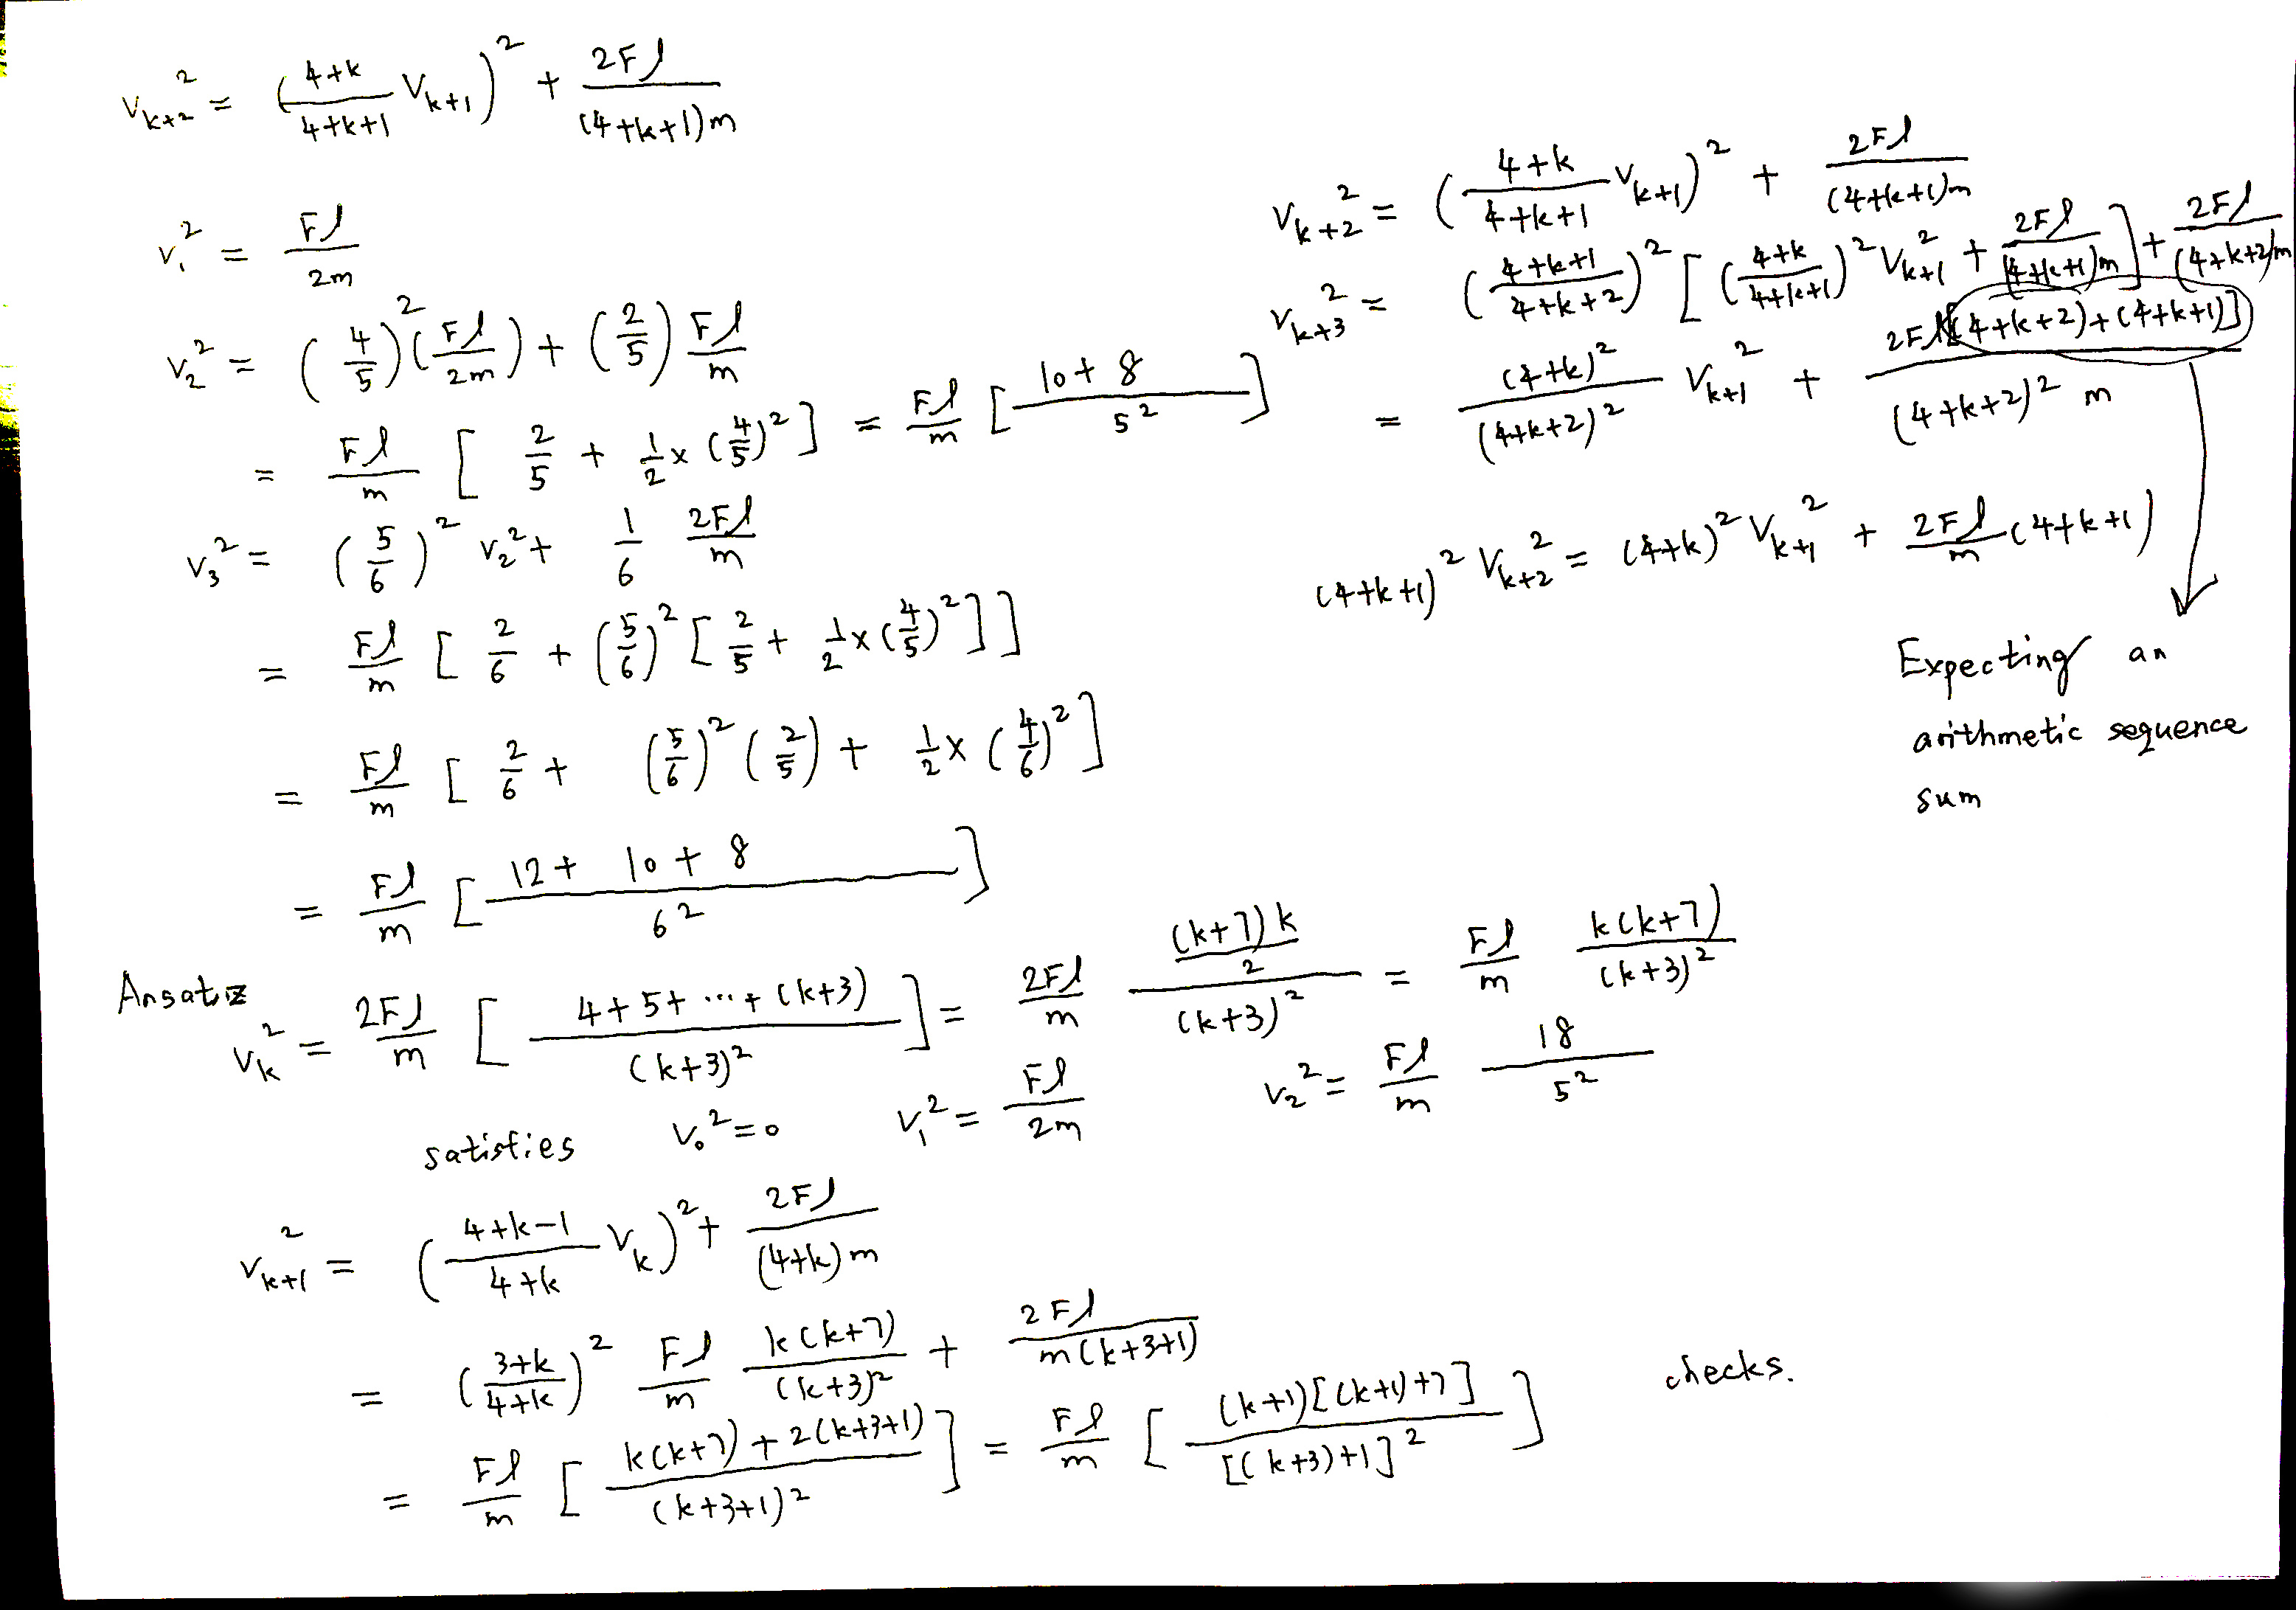
\includegraphics[width=\textwidth]{Midterm2ReviewHandout_SequenceSol.JPG}
\caption{Solution to Recurrence Relation\label{fig:mymathematicalprocedure} in Exercise~\ref{ex:CoMFoR}}
\end{figure}
\[v_k^2=\frac{Fl}{m}\frac{(k+3)^2+(k+3)-12}{(k+3)^2}\]
The maximum velocity is attained at $k=21$ with $v_{21}=\sqrt{\frac{Fl}{m}\cdot\frac{49}{48}}$.

Alternatively, we can change our perspective of view from the ground frame of reference to the center-of-mass frame of reference. During collisions, the energy with respect to the center-of-mass reference is lost, but the energy of the center of mass retains. Consider the large block $M$ and the first $k$ blocks $m$s. The coordinate is shown in Figure~\ref{fig:mycenterofmassforsol}. The work of $F$ done on the center of mass is equal to $F$ times the distance the center of mass moves from the initial instant to the time this system of $M$ and $k$ blocks $m$s is just about to collide into the $k+1$th block $m$. The velocity before the collision is therefore obtained.
\begin{figure}[h]
\centering
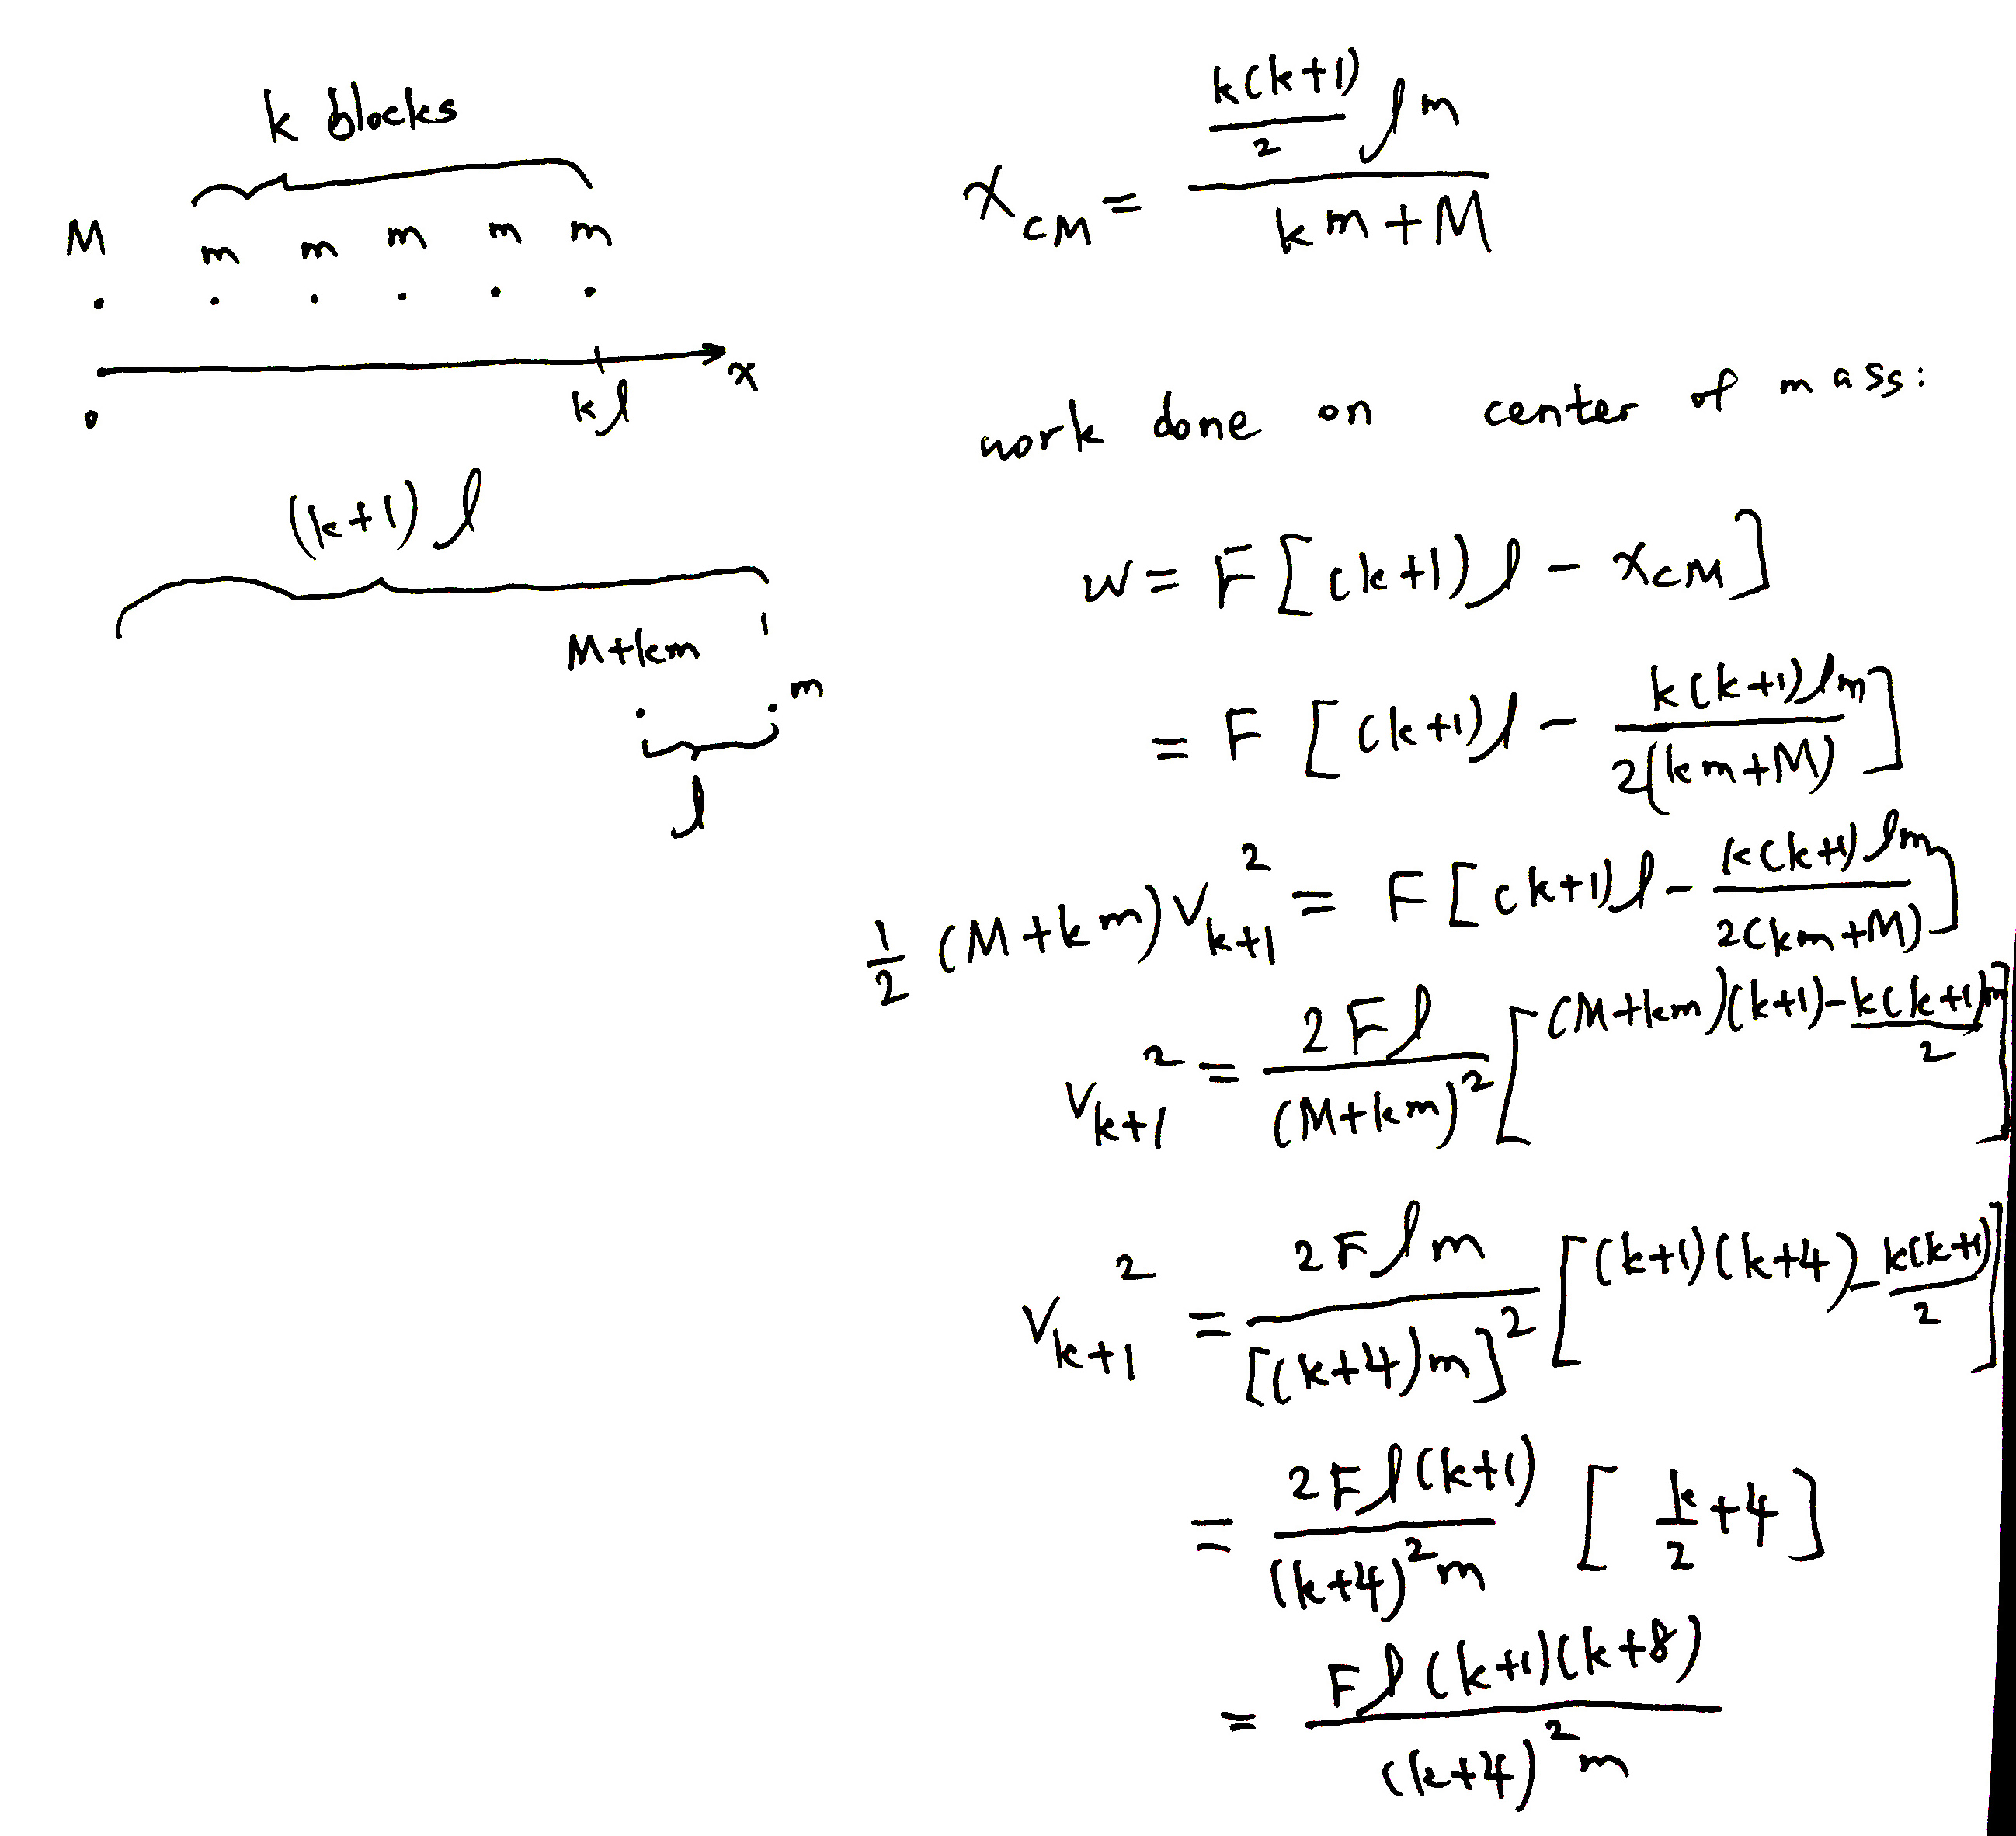
\includegraphics[width=0.6\textwidth]{Midterm2ReviewHandout_CoMFoRSol.JPG}
\caption{Solution using Center-of-Mass Frame of Reference to Exercise~\ref{ex:CoMFoR}\label{fig:mycenterofmassforsol}}
\end{figure}
\end{document}
